\documentclass[tikz]{standalone}
\usetikzlibrary{intersections}
\begin{document}
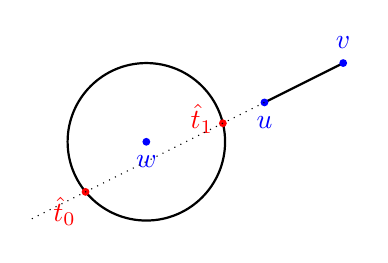
\begin{tikzpicture}
  \coordinate (u0) at (-2,-1);
  \coordinate (u) at (1,0.5);
  \coordinate (v) at (2,1);
  \coordinate (w) at (-0.5,0);

  \draw[thick] (u) -- (v);
  \draw[thick] (w) circle (1);

  \path[name path=line] (u0) -- (v);
  \path[name path=circle] (w) circle (1);
  \path[name intersections={of=line and circle, by={t1,t0}}];

  \node[circle,fill,color=blue,inner sep=1pt,label={[text=blue]-90:\(u\)}] at (u) [] {}; 
  \node[circle,fill,color=blue,inner sep=1pt,label={[text=blue, above]:\(v\)}] at (v) [] {}; 
  \node[circle,fill,color=blue,inner sep=1pt,label={[text=blue]-90:\(w\)}] at (w) [] {}; 

  \node[circle,fill,color=red,inner sep=1pt,label={[text=red, below left]:\(\hat t_0\)}] at (t0) [] {}; 
  \node[circle,fill,color=red,inner sep=1pt,label={[text=red, left]:\(\hat t_1\)}] at (t1) [] {}; 

  \draw[dotted] (u) -- (u0);
\end{tikzpicture}
\end{document}
